\documentclass{beamer}
\usepackage[english]{babel}
\usepackage[utf8]{inputenc}
\usepackage{verbatim}
\usepackage{graphicx}

\begin{document}

\title{Telepathy Echo Protocol Example}
\author{Maksim Melnikau (max\_posedon)}
\institute{Linux Mobile hobbyist\\World of Tanks developer}
\date{\today}
\frame{\titlepage}

\begin{frame}[fragile]
    \frametitle{Let's start}
    \begin{block}{}
    \begin{itemize}
    \item python
    \item gobject
    \item telepathy
    \item telepathy-python
    \end{itemize}
    \end{block}

    \begin{block}{telepathy-foo}
    \begin{verbatim}
DBusGMainLoop(set_as_default=True)
FooConnectionManager()
MainLoop().run()
    \end{verbatim}
    \end{block}
\end{frame}

\begin{frame}[fragile]
    \frametitle{org.freedesktop.Telepathy.Protocol}

    \begin{block}{Properties}
    \begin{itemize}
    \item EnglishName
    \item Parameters
    \item VCardField
    \item Icon
    \end{itemize}
    \end{block}
\end{frame}

\begin{frame}[fragile]
    \frametitle{class Protocol}
    \begin{block}{foo/protocol.py}
    \begin{verbatim}
class Protocol:

    _proto = PROTOCOL
    _english_name = PROTOCOL.capitalize()
    _icon = "im-%s" % PROTOCOL
    _vcard_field = "im-%s" % PROTOCOL
    _mandatory_parameters = {'account': 's'}
    
    def create_connection(self,
        connection_manager, parameters):
        return FooConnection(self, 
            connection_manager, parameters)
    \end{verbatim}
    \end{block}
\end{frame}

\begin{frame}[fragile]
    \frametitle{org.freedesktop.Telepathy.ConnectionManager}

    \begin{block}{Methods}
    \begin{itemize}
    \item GetParameters
    \item ListProtocols
    \item RequestConnection
    \end{itemize}
    \end{block}

    \begin{block}{Signals}
    \begin{itemize}
    \item NewConnections
    \end{itemize}
    \end{block}

    \begin{block}{Properties}
    \begin{itemize}
    \item Protocols
    \item Interfaceds
    \end{itemize}
    \end{block}
\end{frame}

\begin{frame}[fragile]
    \frametitle{class FooConnectionManager}
    \begin{block}{foo/connection\_manager.py}
    \begin{verbatim}
class FooConnectionManager:

    def __init__(self):
        self._implement_protocol(PROTOCOL, FooProtocol)
    \end{verbatim}
    \end{block}
\end{frame}

\begin{frame}[fragile]
    \frametitle{org.freedesktop.Telepathy.Connection}

    \begin{block}{Methods}
    \begin{itemize}
    \item Connect
    \item Disconnect
    \end{itemize}
    \end{block}

    \begin{block}{Properties}
    \begin{itemize}
    \item Status
    \item Interfaces
    \end{itemize}
    \end{block}

    \begin{block}{Signals}
    \begin{itemize}
    \item StatusChanged
    \end{itemize}
    \end{block}
\end{frame}

\begin{frame}[fragile]
    \frametitle{org.freedesktop.Telepathy.Connection.Interface.Contacts}

    \begin{block}{Methods}
    \begin{itemize}
    \item GetContactAttributes
    \end{itemize}
    \end{block}

    \begin{block}{Properties}
    \begin{itemize}
    \item ContactAttributeInterfaces
    \end{itemize}
    \end{block}
\end{frame}

\begin{frame}[fragile]
    \frametitle{org.freedesktop.Telepathy.Connection.Interface.Requests}

    \begin{block}{Methods}
    \begin{itemize}
    \item CreateChannel
    \end{itemize}
    \end{block}

    \begin{block}{Properties}
    \begin{itemize}
    \item Channels
    \item RequestableChannelClasses
    \end{itemize}
    \end{block}
\end{frame}

\begin{frame}[fragile]
    \frametitle{class Connection}
    \begin{block}{foo/connection.py}
    \begin{verbatim}
class FooConnection:

    def Connect(self):
        self.StatusChanged(CONNECTION_STATUS_CONNECTED,
            CONNECTION_STATUS_REASON_REQUESTED)
    def Disconnect(self):
        self.StatusChanged(CONNECTION_STATUS_DISCONNECTED,
            CONNECTION_STATUS_REASON_REQUESTED)

    def GetContactListAttributes(self, interfaces, hold):
        ret = Dictionary(signature='ua{sv}')
        ...
        return ret
    \end{verbatim}
    \end{block}
\end{frame}

\begin{frame}[fragile]
    \frametitle{org.freedesktop.Telepathy.Channel}
    
    \begin{block}{Properties}
    \begin{itemize}
    \item ChannelType
    \item Interfaces
    \end{itemize}
    \end{block}
\end{frame}

\begin{frame}[fragile]
    \frametitle{class FooChannelManager}
    \begin{block}{foo/channel\_manager.py}
    \begin{verbatim}
class FooChannelManager:

    def __init__(self, connection, protocol):
        self.implement_channel_classes(CHANNEL_TYPE_TEXT,
            self._get_text_channel)

    def _get_text_channel(self, props):
        self.__text_channel_id += 1
        path = "TextChannel%d" % self.__text_channel_id
        return FooTextChannel(self._conn, 
            self, props, object_path=path)
    \end{verbatim}
    \end{block}
\end{frame}

\begin{frame}[fragile]
    \frametitle{org.freedesktop.Telepathy.Channel.Type.Text}

    \begin{block}{Methods}
    \begin{itemize}
    \item AcknowledgePendingMessages
    \end{itemize}
    \end{block}
\end{frame}

\begin{frame}[fragile]
    \frametitle{org.freedesktop.Telepathy.Channel.Interface.Messages}

    \begin{block}{Methods}
    \begin{itemize}
    \item SendMessage
    \end{itemize}
    \end{block}

    \begin{block}{Signals}
    \begin{itemize}
    \item MessageSent
    \item MessageReceived
    \end{itemize}
    \end{block}

    \begin{block}{Properties}
    \begin{itemize}
    \item SupportedContentType
    \item PendingMessages
    \end{itemize}
    \end{block}
\end{frame}

\begin{frame}[fragile]
    \frametitle{class FooTextChannel}
    \begin{block}{foo/channel/text.py}
    \begin{verbatim}
class FooTextChannel:
    def SendMessage(self, message, flags):
        gobject.timeout_add(50, self._send_message,
            message, flags, token)

    def _send_message(self, message, flags, token):
        self.MessageSent(message, flags, token)
        gobject.timeout_add(50, self._message_received, 
            str(message[1]['content']))

    def _message_received(self, msg):
        self.MessageReceived(message)
    \end{verbatim}
    \end{block}
\end{frame}

\begin{frame}[fragile]
    \frametitle{Contact List}

    \begin{columns}
    
    \begin{column}{0.37\textwidth}
    \begin{figure}[htb]
    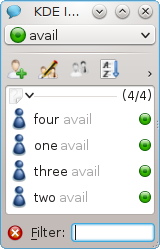
\includegraphics[width=\textwidth]{ktp_list.png}
    \end{figure}
    \end{column}

    \begin{column}{0.63\textwidth}
    \begin{figure}[htb]
    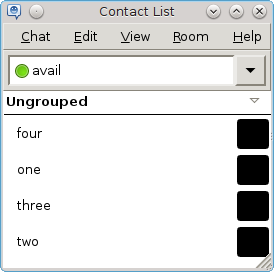
\includegraphics[width=\textwidth]{empathy_list.png}
    \end{figure}
    \end{column}

    \end{columns}
\end{frame}

\begin{frame}[fragile]
    \frametitle{Chat}
    \begin{columns}
    
    \begin{column}{0.46\textwidth}
    \begin{figure}[htb]
    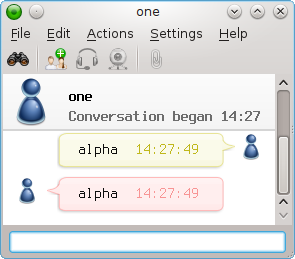
\includegraphics[width=\textwidth]{ktp_msg.png}
    \end{figure}
    \end{column}

    \begin{column}{0.54\textwidth}
    \begin{figure}[htb]
    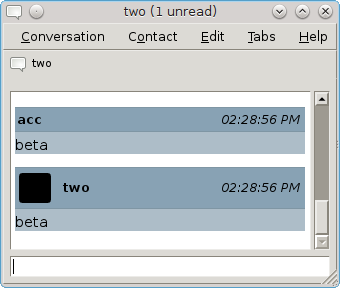
\includegraphics[width=\textwidth]{empathy_msg.png}
    \end{figure}
    \end{column}

    \end{columns}
\end{frame}


\begin{frame}[fragile]
    \frametitle{More Info}
    \begin{itemize}
    \item email: maxposedon@gmail.com
    \item https://github.com/max-posedon/telepathy-foo
    \item https://github.com/max-posedon/telepathy-python
    \item https://github.com/max-posedon/talk-telepathy-echo
    \end{itemize}
\end{frame}

\end{document}
